%% ============================================================
%% 问题二补充：多套备选行程方案 (替换原"基准行程结果"小节)
%% ============================================================

\subsection{多套备选行程方案设计}

题目要求"针对不同出游偏好给出多套可行的备选行程方案"。不同家庭在体力条件、景点偏好和时间观念上存在差异，单一方案难以满足所有需求。本文从偏好维度出发，设计四套差异化方案，覆盖从"高满意度-低可靠度"到"低满意度-高可靠度"的完整偏好谱系。

\subsubsection{方案设计思路}

四套方案的定位如表 \ref{tab:plan_types} 所示。

\begin{table}[H]
\centering
\caption{四套备选方案定位}
\label{tab:plan_types}
\begin{tabularx}{\textwidth}{cclX}
\toprule
方案 & 偏好类型 & 景点数 & 适用场景 \\
\midrule
A & 满意度优先型 & 8 & 精力充沛、希望多打卡景点的家庭 \\
B & 均衡稳健型 & 8 & 一般三口之家，兼顾满意度与时间弹性 \\
C & 轻松休闲型 & 7 & 带幼儿或老人，注重休息节奏的家庭 \\
D & 深度体验型 & 6 & 不追求景点数量，注重游览质量的家庭 \\
\bottomrule
\end{tabularx}
\end{table}

\subsubsection{方案A：满意度优先型}

方案A以最大化景点喜好度为目标，充分利用第一问识别的强联动组合，安排 8 个景点。行程安排如表 \ref{tab:planA} 所示。

\begin{table}[H]
\centering
\caption{方案A行程安排（满意度优先型）}
\label{tab:planA}
\begin{tabular}{cccccc}
\toprule
日期 & 景点 & 喜好度 & 行车/h & 体力负荷 & 理想结束时间 \\
\midrule
第 1 天 & A5 民俗古村 & 7.2 & 1.2 & 2 & 13:42 \\
第 2 天 & A1 古城老街 $\rightarrow$ A10 文创小镇 & 16.2 & 1.2 & 2 & 18:12 \\
第 3 天 & A2 海洋乐园 $\rightarrow$ A8 亲子农庄 & 17.5 & 1.7 & 5 & 20:12 \\
第 4 天 & A4 森林公园 $\rightarrow$ A9 山地观景台 & 15.0 & 2.8 & 5 & 20:18 \\
第 5 天 & A3 滨海浴场 & 7.5 & 0.6 & 1 & 12:06 \\
\bottomrule
\end{tabular}
\end{table}

方案A总满意度为 63.4，但第 3、4 天体力负荷高、缓冲时间仅 0.7--0.8h，抗扰动能力弱。

\subsubsection{方案B：均衡稳健型}

方案B通过拆分高耗时双景点组合来增大每日缓冲。将 A2 海洋乐园和 A4 森林公园各自单独成日，同时在第 1 天和第 5 天安排双景点低负荷组合以保持景点总数不变。行程安排如表 \ref{tab:planB} 所示。

\begin{table}[H]
\centering
\caption{方案B行程安排（均衡稳健型）}
\label{tab:planB}
\begin{tabular}{cccccc}
\toprule
日期 & 景点 & 喜好度 & 行车/h & 体力负荷 & 理想结束时间 \\
\midrule
第 1 天 & A5 民俗古村 $\rightarrow$ A10 文创小镇 & 14.8 & 1.5 & 3 & 18:00 \\
第 2 天 & A1 古城老街 $\rightarrow$ A8 亲子农庄 & 16.9 & 1.5 & 3 & 18:30 \\
第 3 天 & A2 海洋乐园 & 9.2 & 1.6 & 3 & 16:06 \\
第 4 天 & A4 森林公园 & 8.0 & 3.0 & 3 & 17:00 \\
第 5 天 & A3 滨海浴场 $\rightarrow$ A7 环湖湿地 & 14.3 & 0.9 & 2 & 15:54 \\
\bottomrule
\end{tabular}
\end{table}

方案B总满意度为 63.2（与方案A仅差 0.2），但每日最小缓冲时间为 2.5h，体力负荷均衡差从 4 降至 1。

\subsubsection{方案C：轻松休闲型}

方案C以最大化时间弹性为目标，每日最多安排 1 个核心景点（仅第 2、5 天安排联动组合），适合带幼儿或老人的家庭。行程安排如表 \ref{tab:planC} 所示。

\begin{table}[H]
\centering
\caption{方案C行程安排（轻松休闲型）}
\label{tab:planC}
\begin{tabular}{cccccc}
\toprule
日期 & 景点 & 喜好度 & 行车/h & 体力负荷 & 理想结束时间 \\
\midrule
第 1 天 & A10 文创小镇 & 7.6 & 1.0 & 1 & 13:30 \\
第 2 天 & A1 古城老街 $\rightarrow$ A8 亲子农庄 & 16.9 & 1.5 & 3 & 18:30 \\
第 3 天 & A3 滨海浴场 & 7.5 & 0.6 & 1 & 13:06 \\
第 4 天 & A9 山地观景台 & 7.0 & 2.0 & 2 & 14:00 \\
第 5 天 & A5 民俗古村 $\rightarrow$ A7 环湖湿地 & 14.0 & 1.7 & 3 & 16:42 \\
\bottomrule
\end{tabular}
\end{table}

方案C安排 7 个景点，总满意度 53.0，但每日最小缓冲时间为 2.5h，日均行车仅 1.4h。

\subsubsection{方案D：深度体验型}

方案D精选 6 个景点，每个景点给予充足的舒适游览时间，不追求打卡数量。行程安排如表 \ref{tab:planD} 所示。

\begin{table}[H]
\centering
\caption{方案D行程安排（深度体验型）}
\label{tab:planD}
\begin{tabular}{cccccc}
\toprule
日期 & 景点 & 喜好度 & 行车/h & 体力负荷 & 理想结束时间 \\
\midrule
第 1 天 & A1 古城老街 & 8.6 & 1.0 & 1 & 14:00 \\
第 2 天 & A2 海洋乐园 & 9.2 & 1.6 & 3 & 16:06 \\
第 3 天 & A4 森林公园 & 8.0 & 3.0 & 3 & 17:00 \\
第 4 天 & A8 亲子农庄 $\rightarrow$ A10 文创小镇 & 15.9 & 1.5 & 3 & 18:00 \\
第 5 天 & A3 滨海浴场 & 7.5 & 0.6 & 1 & 12:06 \\
\bottomrule
\end{tabular}
\end{table}

方案D总满意度 49.2，但每日最小缓冲时间为 3.0h，且体力负荷均衡差为 2。

\subsubsection{四套方案对比分析}

四套方案的核心指标对比如表 \ref{tab:plan_compare} 所示。

\begin{table}[H]
\centering
\caption{四套备选方案核心指标对比}
\label{tab:plan_compare}
\begin{tabular}{lccccc}
\toprule
方案 & 景点数 & 总满意度 & 日均行车/h & 最大单日负荷 & 最小缓冲/h \\
\midrule
A 满意度优先 & 8 & 63.4 & 1.5 & 5 & 0.7 \\
B 均衡稳健 & 8 & 63.2 & 1.7 & 3 & 2.5 \\
C 轻松休闲 & 7 & 53.0 & 1.4 & 3 & 2.5 \\
D 深度体验 & 6 & 49.2 & 1.5 & 3 & 3.0 \\
\bottomrule
\end{tabular}
\end{table}

由表可知，方案A和方案B的景点数量相同（均为 8 个），总满意度也几乎相同（63.4 vs 63.2），但方案B的最小缓冲时间从 0.7h 提升至 2.5h，体力负荷均衡差从 4 降至 1。这说明通过调整每日景点组合（而非减少景点数量），即可显著提升行程的稳健性。

\begin{figure}[H]
\centering
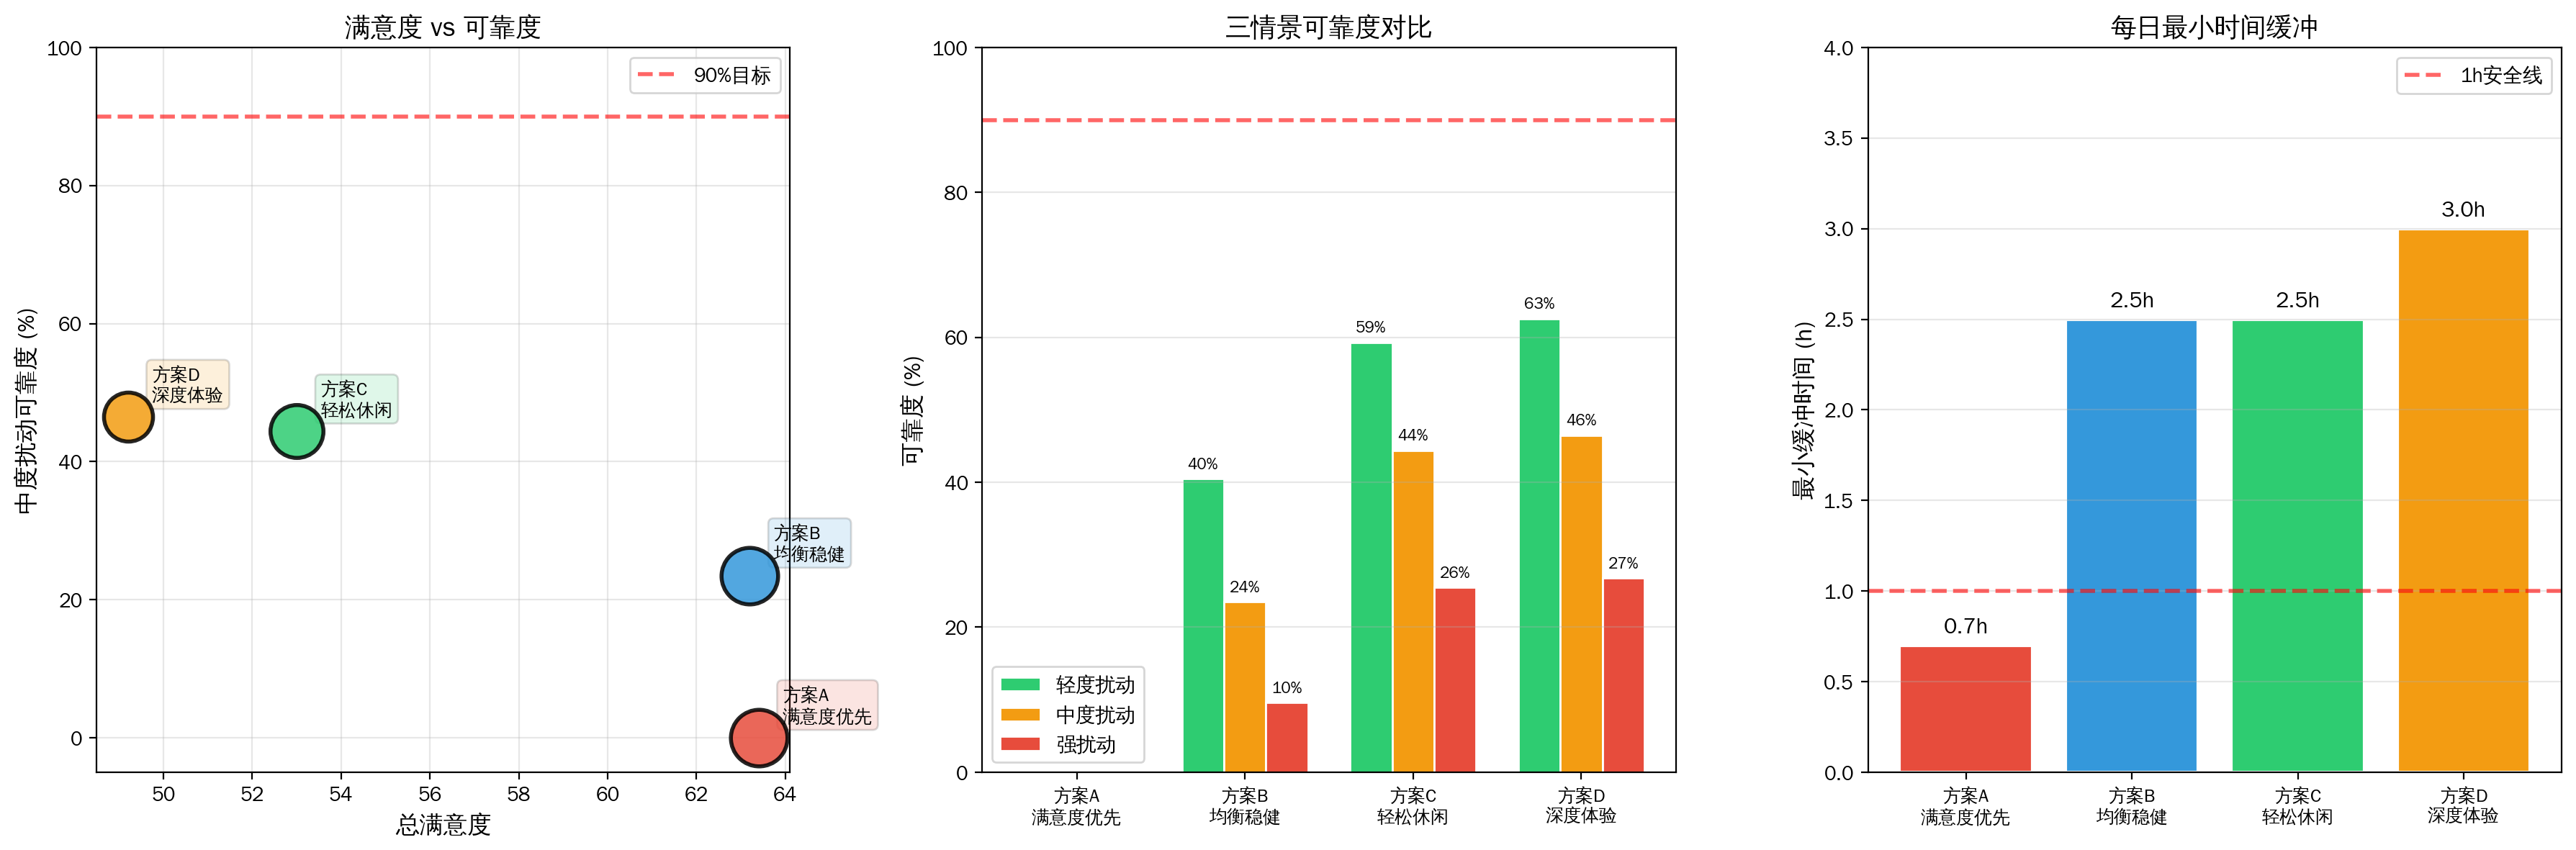
\includegraphics[width=0.92\textwidth]{fig_multi_plans.png}
\caption{四套备选方案多维对比}
\label{fig:multi}
\end{figure}

由图 \ref{fig:multi} 可知，满意度与可靠度之间存在明显的负向权衡关系。方案A满意度最高但可靠度最低（中度扰动下接近 0\%），方案D可靠度最高但满意度最低。方案B在两者之间提供了较优的折中：满意度仅比方案A低 0.2，但中度扰动可靠度提升至 23.5\%。

\begin{figure}[H]
\centering
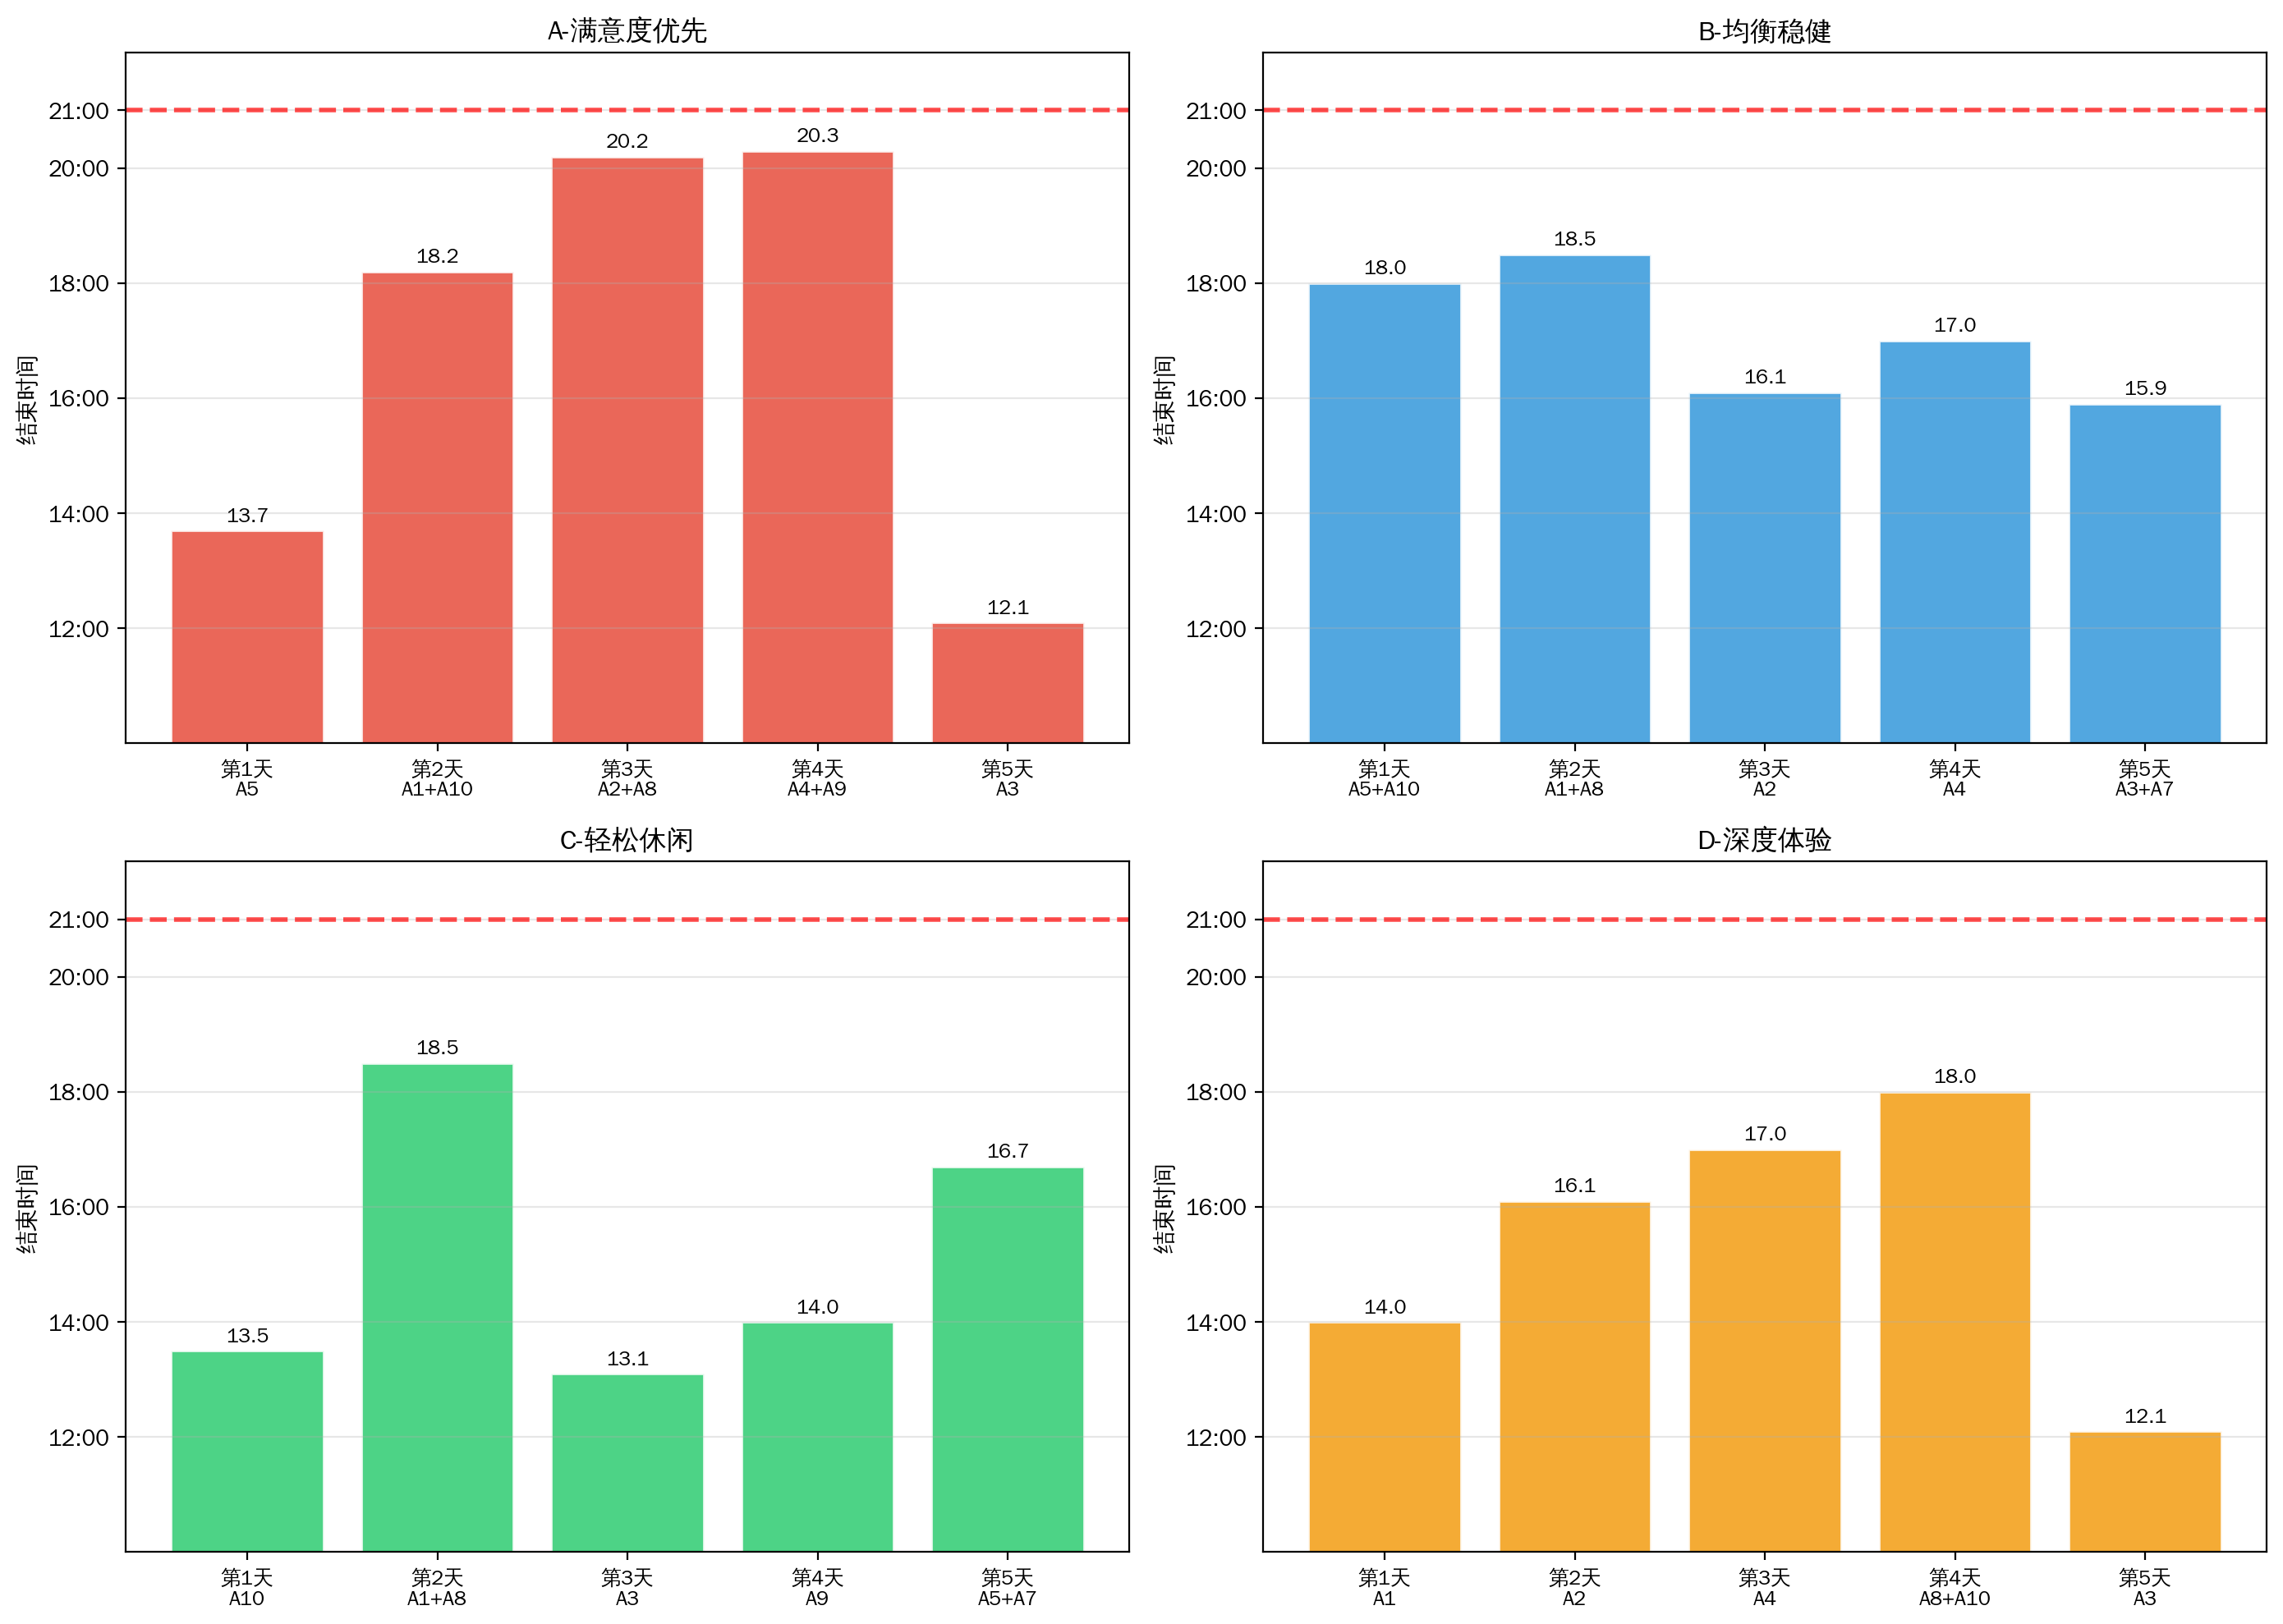
\includegraphics[width=0.88\textwidth]{fig_multi_plans_schedule.png}
\caption{四套方案每日理想结束时间对比}
\label{fig:multi_sched}
\end{figure}

由图 \ref{fig:multi_sched} 可知，方案A的第 3、4 天结束时间接近 21:00 红线，而方案B、C、D均保持了充足的缓冲空间。方案B和方案C虽然景点数量不同（8 vs 7），但每日结束时间分布较为均衡，体现了"不把高负荷景点排在同一天"的编排原则。

\subsubsection{方案推荐建议}

综合考虑满意度、可靠度和家庭适用性，本文给出以下推荐：
\begin{enumerate}[label=(\arabic*)]
    \item \textbf{首选推荐方案B}（均衡稳健型）：满意度与方案A几乎相同，但时间缓冲和体力负荷均衡性显著提升，适合大多数三口之家。
    \item 若家庭中有幼儿或老人，推荐方案C（轻松休闲型），每日不赶路，游览节奏舒缓。
    \item 若家庭特别注重景点体验质量而非数量，推荐方案D（深度体验型），每个景点给予充足游览时间。
    \item 方案A（满意度优先型）仅建议在确信五一期间道路畅通、景点不排队的情况下使用。
\end{enumerate}

\subsection{问题二结论}

本文在无随机扰动条件下，针对不同出游偏好设计了四套备选行程方案。方案A以满意度最大化为目标，安排 8 个景点；方案B通过拆分高耗时叠加组合实现同等景点数量下的稳健性提升；方案C和方案D分别面向轻松休闲和深度体验两种偏好。四套方案覆盖了从"高满意度-低可靠度"到"低满意度-高可靠度"的完整偏好谱系，家庭可根据自身条件选择最适合的方案。


%% ============================================================
%% 同时需要删除或修改的原论文内容:
%% 1. 删除原"基准行程结果"小节中"最终选中8个景点"的单一方案描述
%% 2. 删除原摘要中"编排完整5天详细时序行程"的单一方案表述
%% 3. 在摘要中改为"针对不同出游偏好设计四套备选行程方案"
%% ============================================================
